\chapter{Introduction}

L'objectif de ce projet est de réaliser un processeur xml en C++, en utilisant en plus les outils flex et bison. Ceux-ci nous permettront d'analyser syntaxiquement et sémantiquement le langage xml, afin de créer une grammaire simplifiée. Notre programme a 3 fonctionnalités principales : parser un fichier xml et l'afficher, valider un document xml par rapport à un document xsd, et enfin transformer un document xml avec une feuille de style xsl. En raison du temps qui est imparti pour ce projet, ces fonctionnalités ne couvriront pas toutes les possibilités offertes par le langage xml, afin de réduire le temps de développement de ce programme. \\
Nous l'utiliserons en ligne de commande de la façon suivante :
\begin{description}
    \item[Parsage/affichage du fichier doc.xml~:] ~\\
        \lstinline$xmltool -p doc.xml$
    \item[Validation du fichier doc.xml par rapport au fichier doc.xsd!:] ~\\
        \lstinline$xmltool -v doc.xml doc.xsd$
    \item[Transformation du fichier doc.xml avec la feuille de style doc.xsl~:]~\\
        \lstinline$xmltool -t doc.xml doc.xsl$ \\
\end{description}

Voici l'architecture global de notre programme :

    \begin{figure}[h!]
        \centering
        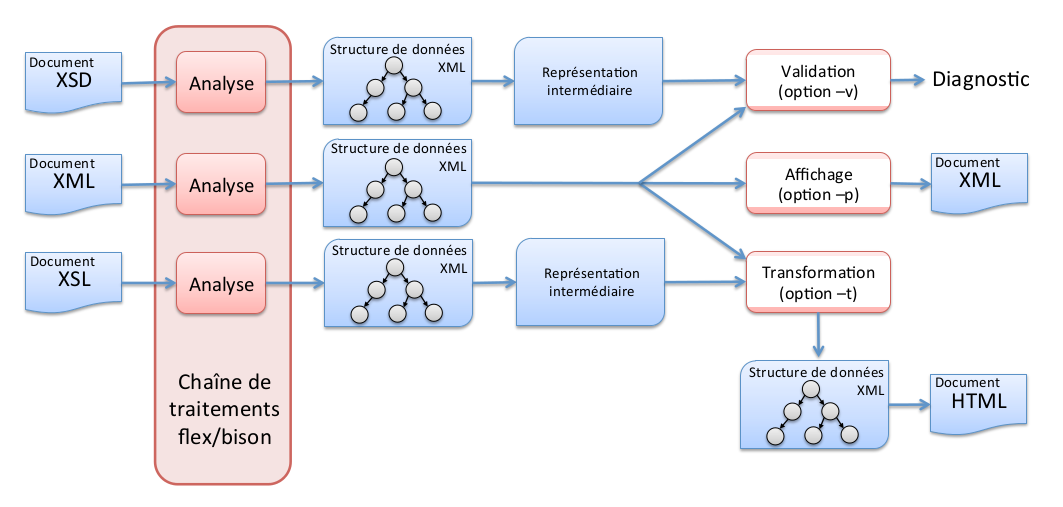
\includegraphics[width=0.8\linewidth]{images/archi.png}
        \caption{Architecture globale}
        \label{classDiagram}
    \end{figure}

La conception sera détaillée plus précisément dans la suite du document.
